\documentclass[
version=last,toc=bib,toc=graduated,toc=index,toc=listof,9pt,openany]{scrbook}
%\pdfminorversion=4
\usepackage[utf8]{inputenc}
\usepackage[ngerman, english]{babel}
\usepackage{dejavu}

\usepackage{ifmtarg}
\usepackage{ifthen}

\usepackage{geometry}
\geometry{%a6paper
paperwidth=125mm, paperheight=168mm, 
portrait,
top=22mm, inner=22mm, outer=20mm, bottom=25mm,
headsep=3mm, footskip=12mm
}

\usepackage{ragged2e} % schöneren Textsatz (Silbentrennung) bei Nicht-Blocksatz
\usepackage{lscape}
\setlength{\parskip}{0pt}

%\pdfminorversion=4


%\usepackage[babel,german=quotes]{csquotes}
\usepackage{relsize}

\clubpenalty=10000 %keine Schusterjungen
 \widowpenalty=10000 
 \displaywidowpenalty=10000 % keine Hurenkinder

\usepackage[letterspace=16]{microtype} %schönerer Textsatz

\usepackage{graphicx} %Bilder

%Dateipfade, wo die Bilder liegen
\graphicspath{{images-print/}{icons/}{extra-pages/}{wallpaper/}}
\usepackage{wrapfig}  % umflossene Logos von Sponsoren mit Multiabsatztexten

\usepackage{tabu}
\usepackage{tabularx}
\usepackage{longtable}
\usepackage[table,cymk]{xcolor}
\usepackage{colortbl}

% PDF-Seiten einbinden
% pdfpages, darf erst nach colortbl geladen werden!
\usepackage{pdfpages}

% PDFs als Hintergrundbilder
% wallpaper, darf erst nach colortbl geladen werden!
\usepackage{wallpaper}
\usepackage{multirow}
\usepackage{booktabs}
\usepackage{array}

\usepackage{mathabx} % für das Rautensymbol in der Speisekarte
\usepackage{textcomp} % degree symbol

\usepackage{refcount} % Berechnung der Seite, auf der sich die Karte befindet

\usepackage[manualmark]{scrpage2}
\pagestyle{scrplain}


\newcommand{\acro}[1]{{\textsmaller{#1}}} % Akronyme

% Überschriften in DejaVu Sans Condensed
\addtokomafont{sectioning}{\fontfamily{DejaVuSansCondensed-TLF}\selectfont}
\addtokomafont{pageheadfoot}{\usefont{T1}{DejaVuSansCondensed-TLF}{m}{n}}
\addtokomafont{pagenumber}{\usefont{T1}{DejaVuSansCondensed-TLF}{m}{n}}


%Titelei
\title{FOSSGIS 2016}
\subtitle{Programm}
\author{FOSSGIS e.V.}
\date{\today}

%\newcommand{\talkroom}{}
\clearscrheadings

% Seitenzahlen
\cfoot[\begin{small}\pagemark\end{small}]{\begin{small}\pagemark\end{small}}
\ofoot[]{}
\ifoot[]{}
\pagestyle{scrplain}

% Durchschuss erhöhen
\linespread{1.15}

% Befehlsdefinitionen einbinden
% neuer Zeitslot
\newcommand{\talktime}{9:99}
\newcommand{\newtimeslot}[1]{\newpage\renewcommand{\talktime}{#1}}

% neuer Zeitslot ohne Seitenumbruch
\newcommand{\newsmalltimeslot}[1]{\renewcommand{\talktime}{#1}}

% \konferenztag initialisieren
\newcommand{\konferenztag}{KeinTag}


% Hintergrund setzen
\def\montag{Montag}
\def\dienstag{Dienstag}
\def\mittwoch{Mittwoch}
\newcommand{\setpagebackground}{ %
	\ifthenelse{\equal{\konferenztag}{\montag}}{ %
		\ifthispageodd{\ThisCenterWallPaper{1.0}{montag-ungerade}}{\ThisCenterWallPaper{1.0}{montag-gerade}}%
	}{}
	\ifthenelse{\equal{\konferenztag}{\dienstag}}{ %
		\ifthispageodd{\ThisCenterWallPaper{1.0}{dienstag-ungerade}}{\ThisCenterWallPaper{1.0}{dienstag-gerade}}%
	}{}
	\ifthenelse{\equal{\konferenztag}{\mittwoch}}{ %
		\ifthispageodd{\ThisCenterWallPaper{1.0}{mittwoch-ungerade}}{\ThisCenterWallPaper{1.0}{mittwoch-gerade}}%
	}{}
}


% Titeltabelle setzen
\newcolumntype{Y}[1]{>{\RaggedRight\arraybackslash}p{#1}}

%% Längen für Sponsorenbox und Titelboxen
\newcommand{\gruenerhs}{Grüner Hörsaal}
\newlength{\titleboxwidth}
\setlength{\titleboxwidth}{\textwidth}
\advance\titleboxwidth by -6pt
\newcommand{\setabstract}[6]{
	% 1. Sprecher
	% 2. Titel
	% 3. Untertitel
	% 4. Abstract (Text)
	% 5. Farbe
	% 6. Raum
	\thispagestyle{scrheadings} 
	\setlength\tabcolsep{0pt}
	% \setlength{\fboxsep}{0pt}
	\noindent\fcolorbox{white}{#5}{\parbox{\titleboxwidth}{%
		\noindent\begin{tabu}{X[5L]r}
			\isspeakerempty{#1}{#2}{#6}
			\issubtitleempty{#3}
		\end{tabu}%
	}}
	%
	\isabstractempty{#4}%
	\ifthenelse{\equal{#6}{\gruenerhs}}%
		{}% bei Grüner HS keinen Seitenhintergrund setzen
		{\setpagebackground%
	}
	\vspace{0.5em}% Abstand zum nächsten Talk, auch wenn es keinen Abstract gibt
	\setlength\tabcolsep{6pt} % Spaltenpadding wieder auf Default setzen
}

% Setzen des Referenten, falls vorhanden
% Wir gehen davon aus, dass es einen Untertitel nur dann gibt, wenn es auch einen Referenten gibt
\makeatletter
\newcommand{\isspeakerempty}[3]{%
	% Arguments:
	% 1. speaker
	% 2. title
	% 3. room
	\@ifmtarg{#1}{%
			\par\noindent\large \sectfont #2% % Titel
			&
			#3, \talktime
			\tabularnewline
		}
		{
			\emph{#1} % Sprecher
			&
			\talktime
			\tabularnewline
			{\par\noindent\large \sectfont #2}% % Titel
			&
			#3
			\tabularnewline
		}
		
}
\makeatother

% Setzen des Untertitels
% muss ausgelagert und durch \makeatletter umgeben sein
\makeatletter
\newcommand{\issubtitleempty}[1]{%
	\@ifnotmtarg{#1}{\multicolumn{2}{Y{\linewidth}}{\vspace{-0.6em} \noindent\bfseries \normalsize \sectfont #1}\tabularnewline}
}
\makeatother

% Setzen des Abstracts, falls vorhanden
% muss ausgelagert und durch \makeatletter umgeben sein
\makeatletter
\newcommand{\isabstractempty}[1]{%
		\vspace{0.5em}\newline%
		#1 \par% % Abstract
		\vspace{1.5em}% Abstand zum nächsten Talk, auch wenn es einen Abstract gibt
}
\makeatother

% Farben definieren
%\definecolor{eins}{cmyk}{ 0 .18 .06 .10}
\definecolor{eins}{cmyk}{ 0 .13 .04 .08}
\definecolor{zwei}{cmyk}{ .1 0 .17 .05}
\definecolor{hellorange}{cmyk}{ 0 0.13 0.35 0.03}
%\definecolor{aula}{cmyk}{ 0.2 0 0.05 0.13}
\definecolor{aula}{cmyk}{ 0.13 0 0.04 0.11}
\definecolor{geoblau}{cmyk}{ 0.2 .02 0 .01}
\definecolor{dezentrot}{cmyk}{ 0 .17 0.21 .04}
\definecolor{hellgelb}{cmyk}{ 0 .02 0.26 0}
\definecolor{hellgruen}{cmyk}{ 0.05 .0 0.17 0.05}

% Abstract Grüner HS
\newcommand{\abstractGruen}[4]%
{%
	\setabstract{#1}{#2}{#3}{#4}{hellgruen}{Grüner HS}
}

% Abstract GI Studio
\newcommand{\abstractGiStudio}[4]%
{%
	\setabstract{#1}{#2}{#3}{#4}{hellgelb}{GI-Studio}
}

% Abstract Audimax
\newcommand{\abstractAudimax}[4]%
{%
	\setabstract{#1}{#2}{#3}{#4}{geoblau}{Audimax}
}

% Abstract Expoforum
\newcommand{\abstractExpo}[4]%
{%
	\setabstract{#1}{#2}{#3}{#4}{hellorange}{Expoforum}
}

% Workshop STUDLAB
\newcommand{\workshopbox}[3]%
{%
	% 1. Titel
	% 2. Referent
	% 3. HS-Nummer
	\setlength\tabcolsep{0pt}
	\noindent\fcolorbox{white}{dezentrot}{\parbox{\titleboxwidth}{%
			\noindent
			\begin{tabu}{X[5L]r}
				\emph{#2} % Sprecher
				&
				\talktime
				\tabularnewline
				{\noindent\large \bfseries #1}% % Titel
				&
				HS\,#3
				\tabularnewline
			\end{tabu}
		}
	}
	\setlength\tabcolsep{6pt} % Spaltenpadding wieder auf Default setzen
}

% viel zu lang
\newcommand{\zulang}{Dieser Text ist viel zu lang. Dieser Text ist viel zu lang. Dieser Text ist viel zu lang. Dieser Text ist viel zu lang. Dieser Text ist viel zu lang. Dieser Text ist viel zu lang. Dieser Text ist viel zu lang. Dieser Text ist viel zu lang. Dieser Text ist viel zu lang. Dieser Text ist viel zu lang. Dieser Text ist viel zu lang. Dieser Text ist viel zu lang. Dieser Text ist viel zu lang. Dieser Text ist viel zu lang. }

%% Längen für Sponsorenbox
\newlength{\fboxwidth}
\setlength{\fboxwidth}{\textwidth}
\advance\fboxwidth by -9pt
%% Sponsorenbox
%% 1. Logo
%% 2. Logobreite
%% 3. negativer vspace nach Logo
%% 4. Text
\newcommand{\sponsorenbox}[4]{%
	\setlength{\fboxsep}{4.5pt}
	\noindent\fcolorbox{gray}{white}{\parbox{\fboxwidth}{
			\begin{floatingfigure}[r]{#2}
				\centering
				\includegraphics[width=#2]{#1}
				\vspace{#3}
			\end{floatingfigure}		
			
			\noindent #4
		}}
		\setlength{\fboxsep}{3pt}
	}


\begin{document}
\lsstyle
\usefont{T1}{DejaVuSansCondensed-TLF}{m}{n}
 
% Schneidemarken
% Befehl zum Aufrufen definieren
\newcommand{\cropmarkswallpaper}{%
\CenterWallPaper{1.0}{crop-marks}%
}
\cropmarkswallpaper

\begin{titlepage}
\ClearWallPaper

\includepdf{deckseite-vektor-mit-schnittmarken}
\cropmarkswallpaper
\end{titlepage}

\selectlanguage{ngerman}
\section*{Inhalt}

\vspace*{0.35em}%
\noindent Workshops am Montag \dotfill \pageref{montag-workshops}

\vspace*{0.35em}%
\noindent Workshops am Dienstag \dotfill \pageref{dienstag-workshops}

\vspace*{0.35em}%
\noindent Workshops am Mittwoch \dotfill \pageref{mittwoch-workshops}

\vspace*{0.35em}%
\noindent Vorträge am Montag \dotfill \pageref{montag}

\vspace*{0.35em}%
\noindent Vorträge am Dienstag \dotfill \pageref{dienstag}

\vspace*{0.35em}%
\noindent Dialoge am Amphitheater \dotfill \pageref{social-event}

\vspace*{0.35em}%
\noindent Vorträge am Mittwoch \dotfill \pageref{mittwoch}

\vspace*{0.35em}%
\noindent Impressum \dotfill \pageref{impressum}

\newpage
\section*{Willkommen zur FOSSGIS-Konferenz 2016 in Salzburg!} \label{welcome}
FOSSGIS ist eine Abkürzung für freie und Open-Source-Software für Geoinformationssysteme.
Die FOSSGIS"=Konferenz ist im DACH-Raum die führende Konferenz zu diesem Thema und findet erstmalig in Österreich statt.

Die FOSSGIS-Konferenz 2016 wird vom gemeinnützigen FOSSGIS e.V und der OpenStreetMap-Community gemeinsam
mit dem AGIT-Tagungsbüro in Zusammenarbeit mit dem Z\_GIS Fachbereich Geoinformatik an der Universität Salzburg organisiert.

Ziel der jährlich stattfindenden Konferenz ist die Verbreitung von Freier und Open-Source-Software für Geoinformationssysteme.
In den nächsten drei Tagen können Sie die Gelegenheit nutzen, sich mit Anwendern und Entwicklern auszutauschen,
sowie neuste Informationen zu Anwendungs- und Arbeitsmöglichkeiten zu bekommen. Im EXPO-Foyer werden Firmen und Projekte ihr Know\-how präsentieren.

Die FOSSGIS-Konferenz findet am Standort der Naturwissenschaftlichen Fakultät in der Hellbrunnerstraße 34 statt.
% Gebäudeinformationen entnehmen Sie bitte dem Standplan im Heft.

\newpage
% hier Goldsponsor einbinden

% Definitionen und Befehle
\newcolumntype{Z}[1]{>{\RaggedRight\arraybackslash}p{#1}}%
\newcolumntype{C}[1]{>{\Centering\arraybackslash}p{#1}}%
\newcommand{\talk}[2]%
{%
	& \textbf{#1} \newline \emph{#2}
}%
% Titel -- Redner


\newcommand{\workshop}[3]%
{%
	\workshopbox{#1}{#2}{#3}
}%

\newcommand{\otherevent}[1]%
{%
	& \textbf{#1}
}%

\newcommand{\aulaevent}[2]%
{%
	&
	\multicolumn{3}{c}{
		\textbf{#1} (Aula) \par \emph{#2}
	}
}%

\newcommand{\coffeespace}{\vspace{0.4em}}
\newcommand{\workshopspace}{\vspace{0.5em}\\}

% Farben definieren
\definecolor{commongray}{gray}{.9}
%\vspace{-1.2em}
\renewcommand{\arraystretch}{1.4}


\newpage
\section*{Workshops am Montag}\label{montag-workshops}%a
	\newsmalltimeslot{15:00 bis 16:30}%
	% Hack, um Einrücken des ersten Workshops wieder rückgängig zu machen
	\RaggedRight
	\noindent\workshop{GraphHopper-Workshop}{Peter Karich}{432}\workshopspace
	\noindent\workshop{QGIS-Grundlagen}{Otto Dassau}{3004}\workshopspace
	\newsmalltimeslot{17:00 bis 18:30}
	\noindent\workshop{Datenmodellierung mit PostgreSQL/PostGIS für QGIS}{Bernhard Ströbel}{432}\workshopspace
	\noindent\workshop{Einführungsworkshop OpenLayers 3}{Marc Jansen}{3004}\workshopspace
% 	
\newpage
\section*{Workshops am Dienstagvormittag}\label{dienstag-workshops}
	\newsmalltimeslot{09:00 bis 10:30}
	\noindent\workshop{OpenStreetMap-Daten finden mit der Overpass-API}{Roland Olbricht}{432}\workshopspace
	\noindent\workshop{PostGIS für Einsteiger}{Astrid Emde}{3004}\workshopspace
	\newsmalltimeslot{11:00 bis 12:30}
	\noindent\workshop{Das neue GRASS-Plugin in QGIS}{Otto Dassau}{432}\workshopspace
	\noindent\workshop{Einführung in die Geodatenverarbeitung mit Python}{Christian Strobl}{3004}\workshopspace

\newpage
\section*{Workshops am Dienstagnachmittag}
	\newsmalltimeslot{13:30 bis 15:00}
	\noindent\workshop{MapFish Print 3 -- Maps, Templates und Reports}{Tobias Sauerwein}{432}\workshopspace
	\noindent\workshop{Mapbender 3}{Astrid Emde}{3004}\workshopspace
	\newsmalltimeslot{15:30 bis 17:00}
	\noindent\workshop{Projektionsmanagement in QGIS}{Class Leiner}{432}\workshopspace
	\noindent\workshop{GeoServer advanced}{Daniel Koch}{3004}\workshopspace

\newpage
\section*{Workshops am Mittwoch}\label{dienstag-workshops}
	\newsmalltimeslot{09:00 bis 10:30}
	\noindent\workshop{Grafische Prozessmodellierung in QGIS}{Class Leiner}{432}\workshopspace
	\noindent\workshop{WebGIS-Anwendungen erstellen mit der 3. Generation von GeoExt}{Christian Mayer}{3004}\workshopspace
	\newsmalltimeslot{10:30 bis 12:00}
	\noindent\workshop{Turf.js – Geoverarbeitung im Browser}{Numa Gremling}{432}\workshopspace
	\noindent\workshop{Karten publizieren mit QGIS Server und QGIS cloud}{Marco Hugentobler, Pirmin Kalberer}{3004}\workshopspace

\newpage
\ifthispageodd{\ThisCenterWallPaper{1.0}{montag-ungerade}}{\ThisCenterWallPaper{1.0}{montag-gerade}}
\section*{Vorträge am Montag}\label{montag}
\noindent\begin{center}
	\noindent\begin{longtabu}{lZ{2.93cm}Z{2.93cm}}
		& \multicolumn{1}{c}{\cellcolor{geoblau} Audimax}
		& \multicolumn{1}{c}{\cellcolor{hellgruen} Grüner HS} \tabularnewline
		\endhead
		10:30
		\talk{}{}
		\talk{Was sind "`Open"' Source, Data und Standards -- und wie funktioniert das?}%
		  {Arnulf Christl, Frederik Ramm, Dominik Helle}\coffeespace
		\coffeespace\tabularnewline
		\rowcolor{commongray}
		12:00 & \multicolumn{2}{c}{%
			\parbox[c]{24pt}{%
				
\includegraphics[height=10pt]{cafe}%
			}
			Pause} \tabularnewline
		13:00
		\talk{Eröffnungs\-veranstaltung}{Marco Lechner}
		\talk{}{}
		\tabularnewline
		13:30
		\talk{Jenseits von Mercator}{Christoph Hormann}
		\talk{}{}
		\coffeespace\tabularnewline
		14:00
		\talk{GIS Lightning Talks 1}{}
		\talk{}{}
		\coffeespace\tabularnewline
		\rowcolor{commongray}
		14:30 & \multicolumn{2}{c}{%
			\parbox[c]{24pt}{%
				
\includegraphics[height=10pt]{cafe}%
			}
			Kaffeepause} \tabularnewline
	\end{longtabu}

\newpage
\ifthispageodd{\ThisCenterWallPaper{1.0}{montag-ungerade}}{\ThisCenterWallPaper{1.0}{montag-gerade}}
	\noindent\begin{longtabu}{lZ{2.93cm}Z{2.93cm}}
		& \multicolumn{1}{c}{\cellcolor{hellgruen} Grüner HS}
		& \multicolumn{1}{c}{\cellcolor{hellgelb} GI-Studio} \tabularnewline
		\endhead
		15:00
		\talk{GIS in der Cloud}{Till Adams}
		\talk{OpenStreetMap und Wikidata}{Michael Maier}
		\coffeespace\tabularnewline
		15:30
		\talk{Freie \mbox{(Geo-)}\newline Daten mit freier (Geo-)Software}{Till Adams}
		\talk{Die Karte verändert sich -- OSM Carto}{Michael Glanznig}
		\coffeespace\tabularnewline
		16:00
		\talk{Schadstoffeinlei\-tungen verfolgen}{Gerhard Genuit\coffeespace}
		\talk{SciGRID}{Wided Medjroubi}
		\coffeespace\tabularnewline
		\rowcolor{commongray}
		16:30 & \multicolumn{2}{c}{%
			\parbox[c]{24pt}{%
				
\includegraphics[height=10pt]{cafe}%
			}
			Kaffeepause} \tabularnewline
		17:00
		\talk{Neues in \mbox{Metador 2.1}}{Axel Schaefer}
		\talk{Automatische Edits und Importe in OSM}{Frederik Ramm}
		\coffeespace\tabularnewline
		17:30
		\talk{Neue Funktionen in QGIS 2.10--2.16}{Marco Hugentobler}
		\talk{Braucht OSM Flächen und Kanten?}{Roland Olbricht}
		\coffeespace\tabularnewline
		18:00
		\talk{Neues von \mbox{MapProxy}}{Oliver Tonnhofer}
		\talk{OSM Lightning Talks}{}
		\coffeespace\tabularnewline
		\rowcolor{commongray}
		18:30 &
		\multicolumn{2}{c}{%
			\textbf{Anwendertreffen/BoFs} (siehe Seite \pageref{bof-montag})}
		\tabularnewline
	\end{longtabu}
	\enlargethispage{0.5em}
\end{center}

\renewcommand{\arraystretch}{1}
\justify
% 10:30
\renewcommand{\konferenztag}{\montag}
\newsmalltimeslot{10:30}
%
\abstractGruen{Arnulf Christl, Frederik Ramm,\newline Dominik Helle\coffeespace}{Was sind "`Open"' Source, Data und Standards -- und wie funktioniert das?}{}{Open Source
hat viele Facetten -- und es ranken sich inzwischen ebenso viele Mythen darum. Was davon richtig ist und was nicht stellen
wir in einer kurzen Einführung zusammen. Was sind Open Data und Open Standards, welche Gemeinsamkeiten gibt es und wo
unterscheiden sie sich. Der Vortrag richtet sich an alle, die mit Open Source, Open Data oder Open Standards bisher
noch wenig Kontakt hatten und die Grundlagen verstehen möchten.

Open Source ist auf der einen Seite ein Entwicklungsmodell und auf der anderen ein Lizenzmodell.
Zusammen bilden sie eine Kultur offener Entwicklungsgmemeinschaften, die höchst effektiv arbeiten. Diese Kultur ist
um ein Vielfaches effektiver, als proprietäre Modelle es je sein können. Ein einfaches Beispiel: Das Betriebssystem
des Herstellers Apple basiert auf dem Open-Source-Unix Free\-BSD. Es gibt halt einfach nichts besseres, und es selbst
herzustellen wäre unendlich teuer, sogar der hyper-pro\-prietäre Hersteller Apple hat das eingesehen.

Der Vortrag stellt die Geschichte der Entwicklung von Open Source vor und geht auf wichtige Grundlagen ein.
%%% Rest weggekürzt, dann ist es solange wie 2015.
% 
% Ziel des FOSSGIS e.V. und der OSGeo ist die Förderung und Verbreitung freier Geographischer Informationssysteme (GIS) im
% Sinne Freier Software und Freier Geodaten. Dazu zählen auch Erstinformation und Klarstellung von typischen Fehlinformationen
% über Open Source und Freie Software, die sich über die Jahre festgesetzt haben.%
}
%
% 13:00
\newtimeslot{13:00}%
\abstractAudimax{Marco Lechner}{Eröffnungsveranstaltung der FOSSGIS-Konferenz 2016}{}%
{Begrüßung durch den Veranstalter der Konferenz (FOSSGIS e.V.) und Grußworte der gastgebenden Universität vertreten durch Herrn Bernhard Zagel}
%
% 13:30
\newsmalltimeslot{13:30}
\abstractAudimax{Christoph Hormann}{Jenseits von Mercator}{}{Karten im OpenStreetMap-Umfeld werden fast immer in
Mercator-Projektion produziert.  Diese prägt durch ihre Verbreitung nicht nur in OpenStreetMap, sondern auch in
so gut wie allen anderen globalen Internet-Kartendiensten unser Verständnis von Geographie und Kartographie in einem erheblichen Ausmaß.

Dieser Vortrag erläutert die Vor- und Nachteile dieser Projektion, insbesondere auch den Einfluss, den diese auf die Datenerfassung
in OpenStreetMap hat. Es werden verschiedene Alternativen mit ihren möglichen Anwendungsfeldern vorgestellt sowie die praktischen
Schwierigkeiten beim Umgang mit Projektionen und der Umrechnung zwischen verschiedenen Koordinatensystemen erläutert.}
%
% 14:00
\newtimeslot{14:00}
\abstractAudimax{}{GIS Lightning Talks 1}{}{\vspace{-2em}
	\begin{itemize}
		\RaggedRight
		\setlength{\itemsep}{-2pt} % Aufzählungspunktabstand auf 0
		\item \emph{Niko Krismer}: Interaktive Karten und HTTP/2
		\item \emph{Doris Silbernagl}: OSMGenie – Expertensystem für OpenStreetMap-Tags
		\item \emph{Dietmar Seifert}: Idee eines POI-Datenabgleichs
		\item \emph{Bernhard Ströbl}: Erste Hilfe bei QGIS
	\end{itemize}
	\justifying
	}
\vspace{1\baselineskip}
\sponsorenbox{102-geoinfo}{0.38\textwidth}{2}{%
\textbf{Silbersponsor}\\
Die GEOINFO IT AG verbindet die Leidenschaft für Geoinformationen mit der
Begeisterung für Softwaretechnologien. Aus den Ideen unserer Kunden entstehen
innovative Lösungen. Darunter bedürfnisgerechte Fachanwendungen für Infrastruktur,
Sicherheit, Vegetation und Landwirtschaft. Wir machen umfangreiche Geoinformationen einfach und zielgruppengerecht zugänglich.
Das Rückgrat unserer Geodateninfrastrukturen bilden eigene moderne Rechenzentren.
Als einziger Schweizer Anbieter der Branche entwickeln wir zudem selbständig Software-Produkte.
Auch deswegen gehört die GEOINFO IT AG in der Schweiz zu den führenden Anbietern umfassender
Geodateninfrastrukturen.}
%
% 15:00
\newtimeslot{15:00}
\abstractGruen{Till Adams}{GIS in der Cloud - Schönwetterwolke, Gewitter oder reiner Dunst?}{}{%
Das WebGIS-Systeme Desktop-basierten an Funktionalität zunehmend ebenbürtig werden, ist fast schon ein alter Hut.
Doch wie sieht es auf der Serverseite aus?

Ist die Verlagerung von GIS-Architekturen in die Cloud wirklich die allseits Schönwetter-Machende,
problemlos skalierbare Alternative zur klassischen Anmietung eines Servers, wo sind Fallstricke,
wie sieht es mit den Kosten aus und überhaupt, wo landen meine Daten eigentlich?~\dots}

\abstractGiStudio{Michael Maier}{OpenStreetMap und Wikidata}{}{Was Tim-Berners Lee mit dem www begonnen hat (Texte zu verlinken),
wird nun mit dem Öl des 21. Jahrhunderts, den Daten weitergeführt.
Lasst OpenStreetMap ein Teil der Linked Open Data Cloud werden!
%
Zwischen OpenStreetMap und Wikipedia wird bereits rege verlinkt -- Nehmen wir die nächste Stufe in Richtung 
Maschinenlesbarkeit und verlinken auch nach Wikidata -- und zurück!}
%
% 15:30
%TODO kürzen
\newtimeslot{15:30}
\abstractGruen{Till Adams}{Freie (Geo-)Daten mit freier \mbox{(Geo-)Software} \emph{oder} wie kommen Geodaten zum Nutzer?}{}%
{%
Die "`Sentinel-Satelliten"'
(Radar, optische, Infrarot- und Thermalsensoren)
des EU-Copernicus-Programms stehen
als freie Daten bereit, sind aber sowohl groß als auch komplex in der Verarbeitung. Wir zeigen die zeitnahe Prozessierung
mit sen2cor und GRASS GIS, Auswertung und automatisierte Bereitstellung als OGC-Webservices (GeoServer,
OpenLayers3, und BasiGX).}

\abstractGiStudio{Michael Glanznig}%
{Die Karte verändert sich -- der \mbox{Standardstil} openstreetmap-carto}%
{}%
{Alle paar Wochen ist es wieder soweit: ein Mapnik-Update (\emph{osm-carto}), die Karte verändert sich.
Nicht immer sind so große Änderungen wie die Darstellung der Straßen dabei und nicht immer sind
alle von den Änderungen begeistert. Dieser Vortrag versucht ein wenig hinter die Kulissen
der osm-carto-Entwicklung zu blicken und darzustellen in welchem Spannungsfeld sich der Standardstil bewegt.
\enlargethispage{6ex}

Welche Ziele hat osm-carto eigentlich? Wie finden Änderungen den Weg in den Kartenstil?
Wer entscheidet das und wie? Kann ich dazu beitragen? Wie kann ich meinen eigenen Kartenstil erstellen?}

\newtimeslot{16:00}
\abstractGruen{Gerhard Genuit}%
{Schadstoffeinleitungen in Kanäle und Gewässer verfolgen}%
{}%
% Kurzbeschreibung durch manuelle Zusammenfassung entstanden, da der Referent selbst unter dem Zeichenlimit geblieben ist
{Dieser Vortrag besteht aus drei Teilen.
Nach einer Einführung in die Probenahme und Auswertung von Biofilmproben,
wird die Erfassung der Daten in dem \emph{Anlagen- und Indirekteinleiterkataster} (AUIK) der Stadt Bielefeld
vorgestellt. Das AUIK ist eine Eigenprogrammierung mit Java-Frontends und einem
PostGIS-Datenbank\-backend und ist unter der GPL verfügbar.
Der dritte Teil beschäftigt sich mit der GIS-Anbindung in Form von WMS und WFS.
}

\abstractGiStudio{Wided Medjroubi}%
{SciGRID -- ein offenes Referenzmodell europäischer Übertragungsnetze für wissenschaftliche Untersuchungen}%
{}%
{Zentraler Gegenstand  des Projektes SciGRID ist die Entwicklung eines frei verfügbaren
und gut dokumentierten Modells des europäischen Übertragungsnetzes basierend auf
OpenStreetMap. In diesem Beitrag werden das Vorgehen in SciGRID und erste
Ergebnisse präsentiert, wie aus den power-Tags ein Netzmodell entsteht.}

\newtimeslot{17:00}
\abstractGruen{Axel Schaefer}%
{Neues in Metador 2.1}%
{}%
{Metador 2 ist eine OpenSource Lösung zum einfachen Erstellen und Bearbeiten von Metadaten.
Metador~2.1 enthält ein neues Plugin-System, mit dem beispielsweise unterschiedliche Metadatenprofile
einfacher und übersichtlicher erstellt und mit Import- und Exportfunktionen unterstützt werden können.
Der Vortrag stellt die Neuerungen in der kommenden Version 2.1 mit Live-Beispielen vor.}

\abstractGiStudio{Frederik Ramm}%
{Automatische Edits und Importe in OpenStreetMap}%
{}%
{Dieser Vortrag zeigt die Probleme auf, die mit großflächigen automatischen und halb-automatischen Edits in OpenStreetMap einhergehen, und diskutiert Alternativen hierzu. }

\newtimeslot{17:30}
\abstractGruen{Marco Hugentobler}%
{Neue Funktionen in QGIS 2.10--2.16}%
{}%
{Seit der FOSSGIS 2015 in Münster sind vier neue QGIS-Versionen herausgekommen,
jede mit zahlreichen Neuerungen. Der Vortrag stellt ausgewählte neue Features,
vor allem aus den Bereichen Geometrie und Symbolisierung, vor.}

\abstractGiStudio{Roland Olbricht}%
{Braucht OpenStreetMap Flächen und Kanten?}%
{}%
{Modellbildung findet bei OpenStreetMap nicht nur durch die Wahl der Tags statt.
Werden Elemente als Linie oder Fläche erfasst?
Offensichtliche Zweifelsfälle sind Fußgängerzonen in Breiten zwischen Straße und Platz.
Aber auch generell nehmen die meisten Objekte im realen Raum Fläche ein.
Gleichzeitig haben dennoch einige Objekte entweder sehr strikten Liniencharakter wie z.B. Gleise.

In diesem Vortrag werden Werkzeuge vorgestellt,
um ein Kantenmodell zu berechnen, ein Flächenmodell zu berechnen
und um die dabei zutage tretrenden Umstimmigkeiten zu finden.
}


\newtimeslot{18:00}
\abstractGruen{Oliver Tonnhofer}%
{Neues von MapProxy}%
{}%
{Der Vortrag befasst sich mit unbekannten Funktionen, der große Bandbreite an Einsatzmöglichkeiten und der wachsenden Community von MapProxy.}


\abstractGiStudio{}%
{OSM Lightning Talks}%
{}%
{\RaggedRight\vspace{-2em}\begin{itemize}
		\setlength{\itemsep}{-2pt} % Aufzählungspunktabstand auf 0
		\item \emph{Felix Delattre}: Karten, die verändern -- Mapping mit Kindern und Jugendlichen
		\item \emph{Alaa Alhamwi}: Raumzeitliche Analyse und Opti\-mierung urbaner Energiesysteme unter Verwendung von OSM-Daten und QGIS
		\item \emph{Dominik Helle}: Magnacarto -- Einfaches Karten\-styling für MapServer und Mapnik 
	\end{itemize}
	\justifying
	}

\newsmalltimeslot{18:30}
\abstractGruen{Astrid Emde}%
{PostNAS-Suite Anwendertreffen}%
{}%
{PostNAS ist ein Projekt zum Import von ALKIS-Daten über
OGR. Es werden aktuelle Entwicklungen des Projekt vor-
gestellt.}\label{bof-montag}

\newpage
\ThisCenterWallPaper{1.0}{montag-ungerade}
\sponsorenbox{104_geofabrik}{0.53\textwidth}{3}{%
	\textbf{Silbersponsor}\\
	Die Geofabrik GmbH ist ein OpenStreetMap"=Expertenbüro in Karlsruhe. 
	Seit 2007 extrahiert, filtert und verarbeitet die Geofabrik für Sie 
	freie Geodaten, erzeugt Shapefiles, Kartenbilder, Kacheln oder 
	komplette Web-Kartenanwendungen. Die Geofabrik ist spezialisiert 
	auf Dienstleistungen rund um OpenStreetMap, wie Beratung, Datenexport, 
	Server-Setup und Software-Entwicklung.}
\vspace{4\baselineskip}\newline
\sponsorenbox{202_Camp2Camp.png}{0.4\textwidth}{4}{%
\textbf{Bronzesponsor\\Stand im EXPO-Forum}\\
Camptocamp gehört zu den führenden Schweizer Dienstleistern im Bereich von Open-Source-GIS
und ist durch sein Engagement in diversen Open-Source-Communitys international geschätzt.
Unsere Dienstleistungen stützen sich auf über 10 Jahre Erfahrung in der Umsetzung von innovativen (Web-)GIS-Lösungen
für Behörden und Unternehmen und erlauben einen hochwertigen und individuellen Service.}\enlargethispage{1\baselineskip}
\newpage % nötig, sonst sind die Spaltenüberschriften auf der nächsten Seite kaputt

\newpage
\renewcommand{\arraystretch}{1.4}
\ifthispageodd{\ThisCenterWallPaper{1.0}{dienstag-ungerade}}{\ThisCenterWallPaper{1.0}{dienstag-gerade}}
\section*{Vorträge am Dienstag}\label{dienstag}
\noindent\begin{center}
	\noindent\begin{longtabu}{lZ{2.93cm}Z{2.93cm}}
		& \multicolumn{1}{c}{\cellcolor{hellgruen} Grüner HS}
		& \multicolumn{1}{c}{\cellcolor{hellgelb} GI-Studio} \tabularnewline
		\endhead
		09:00
		\talk{GeoPackage, das Shapefile der \mbox{Zukunft}}{Pirmin Kalberer}
		\talk{osm\_address\_db~-- Adressdaten in der OSM-Datenbank}{Christopher Lorenz}
		\tabularnewline
		09:30
		\talk{Umstellung von Übungen auf QGIS}{Michael Paulmann}
		\talk{Vector Tiles from OpenStreetMap}{Manuel Roth}
		\tabularnewline
		10:00
		\talk{Automatische Erkennung der Projektion von Geodaten}{Manfred Egger}
		\talk{Stand der Hausnummern in OSM und Hausnummerauswertung auf regio-osm.de}{Dietmar Seifert}
		\coffeespace\tabularnewline
		\rowcolor{commongray}
		10:30 & \multicolumn{2}{c}{%
			\parbox[c]{24pt}{%
				
\includegraphics[height=10pt]{cafe}%
			}
			Kaffeepause} \tabularnewline
\end{longtabu}

\newpage
\vspace*{6ex}
% Beide Tabellen auf derselben Höhe beginnen lassen. Wenn beide so weit oben wie möglich beginnen,
% sieht es doof aus.
\ifthispageodd{\ThisCenterWallPaper{1.0}{dienstag-ungerade}}{\ThisCenterWallPaper{1.0}{dienstag-gerade}}
	\noindent\begin{longtabu}{lZ{2.93cm}Z{2.93cm}}
		& \multicolumn{1}{c}{\cellcolor{hellgruen} Grüner HS}
		& \multicolumn{1}{c}{\cellcolor{hellgelb} GI-Studio} \tabularnewline
		\endhead
		11:00
		\talk{Betrieb von QGIS in einer heterogenen Client-Server-Umgebung}{Andreas Schmid}
		\talk{Mapillary-Alltag}{Lars Schimmer}
		\tabularnewline
		11:30
		\talk{QGIS meets \mbox{MapProxy}}{Sara Biesel}
		\talk{Leitstellen\-simulator goes OpenStreetMap}{Serhan Şen}
		\tabularnewline
		12:00
		\talk{Die Zugriffszeit auf den QGis-Mapserver um Faktor 100 beschleunigen}{Jörg Habenicht}\coffeespace
		\talk{Turf.js -- Geoverarbeitung im Browser}{Numa Gremling}
		\coffeespace\tabularnewline
		\rowcolor{commongray}
		12:30 & \multicolumn{2}{c}{%
			\parbox[c]{24pt}{%
				
\includegraphics[height=10pt]{restaurant}%
			} 
		Mittagspause bis 13:30} \tabularnewline
\end{longtabu}

\newpage
\ifthispageodd{\ThisCenterWallPaper{1.0}{dienstag-ungerade}}{\ThisCenterWallPaper{1.0}{dienstag-gerade}}
	\noindent\begin{longtabu}{lZ{2.93cm}Z{2.93cm}}
		& \multicolumn{1}{c}{\cellcolor{hellgruen} Grüner HS}
		& \multicolumn{1}{c}{\cellcolor{hellgelb} GI-Studio} \tabularnewline
		\endhead
		13:30
		\talk{Web-basierte \mbox{Geoprozessierung} mit Python und PyWPS}{Jonas Eberle}
		\talk{OpenStreet mal ohne Map}{Frederik Ramm}
		\tabularnewline
		14:00
		\talk{Hybride mobile App-Entwicklung mit Angular}{Arne Schubert}
		\talk{Bezahlte und organisierte Edits -- Vorteile und Gefahren für OSM}{Joachim Kast}
		\tabularnewline
		14:30
		\talk{mapmap.js -- eine kartographische API für interaktive thematische Karten}{Florian Ledermann}
		\talk{Ansätze zur Lokalisierung einer OpenStreetMap-basierten \mbox{Weltkarte}}{Sven Geggus}\coffeespace
		\coffeespace\tabularnewline
		\rowcolor{commongray}
		15:00 & \multicolumn{2}{c}{%
			\parbox[c]{24pt}{%
				
\includegraphics[height=10pt]{cafe}%
			}
			Kaffeepause} \tabularnewline
\end{longtabu}

\newpage
\ifthispageodd{\ThisCenterWallPaper{1.0}{dienstag-ungerade}}{\ThisCenterWallPaper{1.0}{dienstag-gerade}}
	\noindent\begin{longtabu}{lZ{2.93cm}Z{2.93cm}}
		& \multicolumn{1}{c}{\cellcolor{hellgruen} Grüner HS}
		& \multicolumn{1}{c}{\cellcolor{hellgelb} GI-Studio} \tabularnewline
		\endhead
		15:30
		\talk{OpenLayers 3 -- Stand, Neues und Ausblick}{Marc Jansen}
		\talk{OSM Lightning Talks}{}
		\tabularnewline
		16:00
		\talk{\selectlanguage{english}Compiling your application \mbox{together} with OpenLayers~3\selectlanguage{ngerman}}{Tobias Sauerwein}
		\talk{Das ist ja wohl die Höhe!}{Lars Roskoden}
		\tabularnewline
		16:30
		\talk{GeoExt3}{Marc Jansen}
		\talk{Flexible Routenplanung mit \mbox{GraphHopper}}{Peter Karich}
		\tabularnewline
		17:00
		\talk{Datenerfassung und Suchen mit Mapbender3}{Astrid Emde}
		\talk{XPlanung für einen Flächennutzungsplan mit PostGIS und QGIS}{Bernhard Ströbl}\coffeespace
		\coffeespace\tabularnewline
		\rowcolor{commongray}
		17:30 &
		\multicolumn{2}{c}{%
			\textbf{Anwendertreffen/BoFs} (siehe Seite \pageref{bof-dienstag})}
		\tabularnewline
	\end{longtabu}
\end{center}

\renewcommand{\arraystretch}{1}
\justify
\renewcommand{\konferenztag}{\dienstag}
\newtimeslot{09:00}
\abstractGruen{Pirmin Kalberer}%
{GeoPackage, das Shapefile der Zukunft}%
{}%
{Im Februar 2014 hat das Open Geospatial Consortium den GeoPackage Encoding Standard offiziell
freigegeben. Dieses noch junge Format hat sich bereits gut etabliert und wird in zahlreichen GIS-Produkten unterstützt.
In Geo\-Package-Dateien können sowohl Vektor- als auch Rasterdaten mit zugehörigen Metainformation gespei\-chert
werden. Damit können Geodaten einfach ausgetauscht und auch auf mobilen Geräten effizient genutzt werden.}

\abstractGiStudio{Christopher Lorenz}%
{osm\_address\_db -- Adressdaten in der OSM-Datenbank}%
{}%
{Das Projekt osm\_address\_db ermöglicht die Aufbereitung der in OSM vorhandenen Adressdaten. Dazu wurden Shell-
und SQL-Skripte entwickelt, die eine Tabellenstruktur zur Auswertung und Analyse aufbauen.
Im Vortrag wird die Datenstruktur, die benutzten Tools und Technologien als auch die während der
Entwicklung aufgetretenen Probleme eingegangen. Die OSM-Daten werden nach dem Karlsruher Schema analysiert,
dabei finden auch associated\-Street-Relationen Berücksichtigung.
Derzeit befindet sich eine Webanwendung zur Auswertung in Entwicklung.}

\newtimeslot{09:30}
\abstractGruen{Michael Paulmann}%
{Umstellung von Übungen auf QGIS}%
{}%
{Im Modul Grundlagen Geographischer Informationssysteme an der Hochschule für Technik in Stuttgart
sollen die Übungen und die Vorlesung nicht mehr in einem proprietären Geoinformationssystem
stattfinden, sondern in die Open-Source-Software QGIS. Es gibt einen Einblick in die Probleme
die bisher auftraten und den bisherigen Fortschritt, der Prozess ist noch nicht abgeschlossen.
Bis Oktober 2016 soll alles auf QGIS geändert worden sein.}

\abstractGiStudio{Manuel Roth}%
{Vector Tiles from OpenStreetMap}%
{}%
{Das Projekt OSM2VectorTiles bietet einerseits einen Workflow, um selbst Vektor Tiles aus OSM zu erstellen,
und bietet diese andererseits gratis zum Download an. Dies ermöglicht jedem, eine selbst gestaltete Karte der
gesamten Welt zu erstellen und anzubieten, ohne Kenntnisse von PostGIS und Mapnik zu haben.
Die Zuhörer wissen nach unserer Präsentation, wie sie eine selbst gestaltete Karte erstellen
und veröffentlichen können. Zudem können sie die vom OSM2VectorTiles-Projekt zur Verfügung gestellten
Daten verwenden, um ihre Karte auch offline anbieten zu können.}

\newtimeslot{10:00}

\abstractGruen{Manfred Egger}%
{Automatische Erkennung der Projektion von Geodaten}%
{}%
{Das GIS-Tool SHAPEFILE PROJECTIONFINDER wird als Lösungsvorschlag
in Zusammenhang mit Geodaten und
unbekannter Projektion präsentiert. Zielgruppe dieses Programms sind vor
allem Anwender, die mit geringen
Fachkenntnissen zu Koordinatensystemen gelieferte Daten ohne Aufwand in
GIS-Projekte lagerichtig integrieren möchten.}

\abstractGiStudio{Dietmar Seifert}%
{Stand der Hausnummern in OSM und Hausnummerauswertung auf regio-osm.de}%
{}%
%%%% Text von Michael geschrieben
{Es wird der aktuelle Stand der Hausnummernerfassung in OSM in Deutschland, aber auch in anderen EU-Ländern erläutet.
In einigen Ländern wurden die Hausnummern aus verfügbaren Quellen importiert
oder es gibt landesweite Listen zum Datenabgleich, in Deutschland ist die
Situation je nach Bundesland sehr unterschiedlich und in Bewegung.
Die Auswertungsmöglichkeiten auf regio-osm.de werden vorgestellt.}

\newtimeslot{11:00}

\abstractGruen{Andreas Schmid}%
{Betrieb von QGIS in einer hete\-rogenen Client-Server-Umgebung}%
{}%
{Das Amt für Geoinformation des Kantons Solothurn betreibt für die Benutzer der
Kantonsverwaltung QGIS auf einem Linux-Applikationsserver. Für die Integration
der Linux-Anwendung in den via Citrix bereitgestellten Windows"-Desktop, der den
Standard-Arbeitsplatz in der Kantonsverwaltung darstellt, kommt die Open-Source-Lösung X2Go zum Einsatz.
Der Vortrag präsentiert diese Lösung im Detail und geht auf deren Vor- und
Nachteile ein. Zudem vergleicht er sie mit anderen Lösungen, die früher im Einsatz waren und nun abgelöst wurden.}

\abstractGiStudio{Lars Schimmer}%
{Mapillary-Alltag}%
{}%
{Das Ökosystem Mapillary wurde auf der Fossgis 2014 in einem Lightning
Talk schon vorgestellt.
Ich werde aus Benutzersicht meine Erfahrungen aus 18 Monaten Aktivität mit
Mapillary berichten, dieses umfasst über 160\,000 eingereichte Fotos,
diverse genutzte Mobilgeräte, viele besuchte Orte und mehrere Methoden
der Datenbearbeitung. Natürlich werden auch die Pitfalls und Probleme angesprochen, über die
man zwangsweise stolpert.}

\newtimeslot{11:30}

\abstractGruen{Sara Biesel}%
{QGIS meets MapProxy}%
{}%
{Das Bundesamt für Kartographie und Geodäsie entwickelt ein System, um Kartenausschnitte zu speichern und
die Karten offline im Geoinformationssystem QGIS zu laden. Dabei wird ein
Proxyserver MapProxy verwendet, der bei bestehender Internetverbindung
die Karten als Kacheln lokal ablegt. Das ganze System liegt auf einer
portablen, externen Festplatte.}

\abstractGiStudio{Serhan Şen}%
{Leitstellensimulator goes \mbox{OpenStreetMap}}%
{}%
{Das nichtkommerzielle Browserspiel LstSim, ein Rettungsleitstellensimulator, setzte jahrelang auf die Dienste
der Google Maps API. Leider gab es mit der API über einen längeren Zeitraum anhaltende Schwierigkeiten. Es wurde
deshalb schon früh der Vorschlag gemacht, man solle doch "`einfach auf OpenStreetMap wechseln"'. Doch was bedeutet
das überhaupt und wie sieht so ein Wechsel aus? Dieser Vortrag fasst die technischen und organisatorischen
Herausforderungen -- und Chancen -- seit Beginn der Umstellungen Ende 2015 zusammen.}

\newtimeslot{12:00}
\abstractGruen{Jörg Habenicht}%
{Die Zugriffszeit auf den QGis-Mapserver um Faktor 100 beschleunigen.}%
{}%
{Wir benutzen den QGIS-Mapserver, um den Kunden verschiedene Karten im
Webbrowser anzuzeigen. Mit unseren großen Konfigurationsdateien von bis
zu 19MB benötigt der Server beim Erstzugriff zur Berechnung länger als
der Browsertimeout. Mit unserem Tool wird der Timeout verhindert und die
Zugriffszeit 100fach beschleunigt.}

\abstractGiStudio{Numa Gremling}%
{Turf.js – Geoverarbeitung im Browser}%
{}%
{Turf.js ist eine Open Source JavaScript-Bibliothek, die geographische Analysen und Abfragen ermöglicht.
Im Gegensatz zu Web Processing Services (WPS), die eine komplexe serverseitige Infrastruktur erfordern,
arbeitet Turf.js clientseitig mit Daten im GeoJSON-Format. Somit ist Turf.js eine schnell und leicht
umzusetzende Alternative zu komplexen Web-GIS-Lösungen.
Im Vortrag werden klassische Werkzeuge zur Analyse von Geodaten, wie Puffer und Punkt-in-Polygon, aber auch
die Durchführung komplexer Analysen vorgestellt.}

\newtimeslot{13:30}
\abstractGruen{Jonas Eberle}%
{Web-basierte Geoprozessierung mit Python und PyWPS}%
{}%
{Web-basierte Prozessierungsdienste können für eine Vielzahl an Aufgaben verwendet werden und bieten enorme Möglichkeiten,
Nutzer- und Entwicklerfreundliche Geodatendienste aufzubauen. Dies wird an einigen einfachen und komplexen Beispielen gezeigt,
die mit der Software PyWPS im Rahmen der Programmiersprache Python online veröffentlicht worden sind.
Dieser Vortrag liefert anfangs eine Einführung in den Bereich der „Web Processing Services“ und zeigt
zudem das Potential web-basierter Prozessierung mittels WPS im Geodatenbereich auf. }

\abstractGiStudio{Frederik Ramm}%
{OpenStreet mal ohne Map}%
{}%
{Dieser Vortrag erzählt von verschiedenen - realistischen wie auch unrealistischen - Anforderungen,
die potentielle Nutzer abseits von der Kartenerstellung an OpenStreetMap stellen, und skizziert Lösungen und Probleme.}

\newtimeslot{14:00}
\abstractGruen{Arne Schubert}%
{Hybride mobile App-Entwicklung mit Angular}%
{}%
{}

\abstractGiStudio{Joachim Kast}%
{Bezahlte und organisierte Edits - Vorteile und Gefahren für OSM}%
{}%
{}

\newtimeslot{14:30}
\abstractGruen{Florian Ledermann}%
{mapmap.js - Ein kartographisches API für interaktive thematische Karten}%
{}%
{Das an der TU Wien entwickelte API mapmap.js versucht den kartographischen
Visualisierungsprozess in seiner Gesamtheit in einem high-level JavaScript API
abzubilden, wobei jeder Teilaspekt zunächst „einfach funktioniert“, aber bei
Bedarf im Detail an die Notwendigkeiten der jeweiligen Anwendung angepasst werden
kann und somit auch die Entwicklung neuer Visualisierungstechniken erlaubt.}

\abstractGiStudio{Sven Geggus}%
{Ansätze zur Lokalisierung einer Openstreetmap basierten Weltkarte}%
{}%
{Der Vortrag stellt eine vom Renderer unabhängige Methode zur Latinisierung
von OSM-basierten Karten vor. Als Datenquelle dient, wenn möglich, OSM
selbst. Alternativ wird Transkription verwendet, die jedoch viele
Schriftsystem-abhängige Probleme birgt, für die teilweise Lösungen
aufgezeigt werden. Ferner wird auf politische Probleme bei der Lokalisierung
von Karten eingegangen.}

\newtimeslot{15:30}
\abstractGruen{Marc Jansen}%
{OpenLayers 3: Stand, Neues und Ausblick}%
{}%
{}

\abstractGiStudio{TBA}%
{OSM Lightning Talks}%
{}%
{}

\newtimeslot{16:00}
\abstractGruen{Tobias Sauerwein}%
{Faster, smaller, better: Compiling your application together with OpenLayers 3}%
{}%
{}

\abstractGiStudio{Lars Roskoden}%
{Das ist ja wohl die Höhe!}%
{}%
{Darstellung einfacher Möglichkeiten für die Höhenmessung von OSM-Objekten. Vergleich der Vor- und Nachteile.}

\newtimeslot{16:30}
\abstractGruen{Marc Jansen}%
{GeoExt3}%
{}%
{}

\abstractGiStudio{Peter Karich}%
{Flexible Routenplanung mit GraphHopper}%
{}%
{GraphHopper ist ein schneller und flexibler Open Source Routenplaner basierend auf OpenStreetMap Daten,
der sowohl offline auf dem Gerät als auch auf dem Server läuft und schon bei vielen bekannten Organisationen
und Firmen produktiv eingesetzt wird. GraphHopper ermöglicht nicht nur Routing von A nach B, sondern auch
Reichweitenanalyse, Map Matching und vieles mehr.}

\newtimeslot{17:00}
\abstractGruen{Astrid Emde}%
{Datenerfassung und Suchen mit Mapbender3}%
{}%
{Der Vortrag zu Mapbender3 stellt fortgeschrittene Elemente mit erweiterter Konfiguration vor. 
\begin{itemize}
 \item Möglichkeiten der Datenerfassung mit dem Mapbender3 Digitizer
 \item Aufbau von Suchen mit dem SearchRouter (SQL basierte Suchen)
 \item Aufbau von Suchen mit SimpleSearch (Solr basierte Suchen)
\end{itemize}%
}

\abstractGiStudio{Bernhard Ströbl}%
{XPlanung für einen Flächennutzungsplan mit PostGIS und QGIS}%
{}%
{Der Vortrag zeigt die erfolgte Umsetzung des Standards XPlanung für PostGIS und den Zugriff darauf aus
QGIS heraus am Beispiel eines in der Aufstellung befindlichen Flächennutzungsplans. }



% Social Event
\newpage
% \ThisCenterWallPaper{1.0}{schlossgartencafe}
\thispagestyle{empty}
\section*{Dialoge am Amphitheater}
\label{social-event}
Von 18:00 bis 23:00 Uhr finden auf der Terasse des Gebäudes Naturwissenschaften in der Universität Salzburg
die \emph{Dialoge am Amphitheater} zusammen mit dem \emph{Icebreaker} der AGIT statt.
Die Veranstaltung wird sich durch ein offenes Ambiente auszeichnen. Der Eintritt ist im Ticket enthalten.

Als Schlechtwettervariante steht das Foyer der Universität zur Verfügung.

\noindent
\begin{center}
  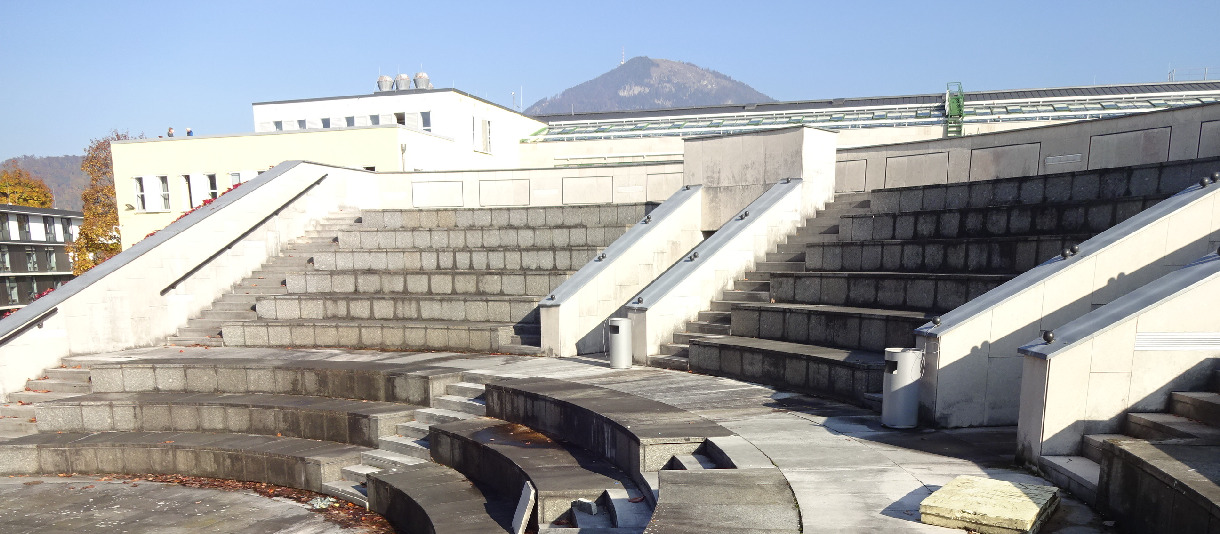
\includegraphics[width=0.95\textwidth]{images_raw/amphitheater-rechts-crop.jpg}
\end{center}

\justifying
\newpage
\renewcommand{\arraystretch}{1.4}
\ifthispageodd{\ThisCenterWallPaper{1.0}{mittwoch-ungerade}}{\ThisCenterWallPaper{1.0}{mittwoch-gerade}}
\section*{Vorträge am Mittwoch}\label{mittwoch}
\vspace{-2ex}
\noindent\begin{center}
	\noindent\begin{longtabu}{lZ{2.93cm}Z{2.93cm}}
		& \multicolumn{1}{c}{\cellcolor{hellgruen} Grüner HS}
		& \multicolumn{1}{c}{\cellcolor{hellgelb} GI-Studio} \tabularnewline
		\endhead
		09:00
		\talk{Zusammenspiel von GIS und CMS}{Nikolaus Dürk}
		\talk{Summer of Code}{Peter Barth}
		\tabularnewline
		09:30
		\talk{Neuerungen im GeoServer}{Daniel Koch}
		\talk{OSM schön gemacht}{Mark Padgham\coffeespace}
		\tabularnewline
		\rowcolor{commongray}
		10:00 & \multicolumn{2}{c}{%
			\parbox[c]{24pt}{%
				
\includegraphics[height=10pt]{cafe}%
			}
			Kaffeepause} \tabularnewline
		10:30
		\talk{Neue Werkzeuge für INSPIRE}{Jürgen Weichand}
		\talk{OSM2World hinter den Kulissen}{Tobias Knerr}
		\coffeespace\tabularnewline
		11:00
		\talk{INSPIRE "`instant"'}{Armin Retterath}
		\talk{Transit-Routing und OSM}{Arndt Brenschede}
		\coffeespace\tabularnewline
		11:30
		\talk{PostNAS-Suite}{Astrid Emde}
		\talk{morituri}{Philip Beelmann}
		\coffeespace\tabularnewline
		\rowcolor{commongray}
		12:00 & \multicolumn{2}{c}{%
			\parbox[c]{24pt}{%
				
\includegraphics[height=10pt]{cafe}%
			}
			Pause bis 13:00} \tabularnewline
		13:00
		\talk{Abschluss\-veranstaltung}{}
		\talk{}{}
		\tabularnewline
		\rowcolor{hellorange}
		\vspace*{-3.2ex} % Abstand reduzieren
		13:30 & \multicolumn{2}{c}{%
			\parbox[c]{24pt}{%
				
\includegraphics[height=10pt]{bar}%
			}
			Sektempfang im EXPO-Forum} \tabularnewline
\end{longtabu}
\end{center}
\renewcommand{\arraystretch}{1}
\justify
\renewcommand{\konferenztag}{\mittwoch}
\newtimeslot{09:00}
\abstractGruen{Carina Waidhofer, Christoph Haselberger}%
{Zusammenspiel von GIS und CMS verdeutlicht die möglichen Folgen einer 2\textdegree-Klimaerwärmung}%
{}%
{Die Linzer Unternehmen X-Net Services GmbH und blp GeoServices GmbH haben die technische Entwicklung
des öffentlich zugänglichen IMPACT2C-Web-Atlas im Auftrag des Climate Service Center Germany realisiert.
Darin werden die möglichen Auswirkungen einer 2\textdegree C"=Klimaerwärmung visualisiert und in einem Dual-Screen
(Map und Pages) für die Allgemeinheit verständlich erklärt. Durch die Darstellung in mehreren Layern
kann die Situation vor und nach einer 2\textdegree C-Klimaerwärmung verglichen werden.}

\enlargethispage{4ex}
\abstractGiStudio{Peter Barth}%
{Summer of Code}%
{}%
{Bereits seit 2008 nimmt das OSM-Projekt als Organisation am Google Summer of Code teil und
hat in diesem Rahmen viele interessante und nützliche Projekte auf den Weg gebracht, aber auch dazu
beigetragen die OSM"=Community zu vergrößern. Der Vortrag gibt einen Überblick über die
vergangenen Jahre, die geleistete Arbeit, die positiven wie negativen Aspekte der Teilnahme, zeigt
aber vor allem auch auf, warum sowohl Studenten als auch OSM von Google Summer of Code profitieren.}

\newtimeslot{09:30}
\abstractGruen{Daniel Koch}%
{Neuerungen im GeoServer}%
{}%
{\dots\ Die sehr aktive GeoServer Community arbeitet laufend an Erweiterungen und Verbesserungen
der Kernsoftware. Dieser Vortrag wird sich einigen (Neu"=)Entwicklungen der jüngeren
Vergangenheit widmen und an praktischen Beispielen den Nutzen vorstellen.

Hierunter fallen u.a. die Importer-Extension zum Hinzufügen von Geodaten in den GeoServer über das Webinterface,
die CSS-Extension zum Stylen von Layern über Cascading Style Sheets,
der WFS-Datenspeicher zur Kaskadierung entfernter WFS-Server,
die Darstellung von Curved Geometries und
die GeoFence-Integration.

Der Vortag wird mit einem Ausblick auf geplante und zukünftige Entwicklungen abschließen.}

\abstractGiStudio{Mark Padgham}%
{OSM schön gemacht}%
{}%
{Das R package, \emph{osmplotr} ermöglicht  die grafisch beliebige Darstellung ausgwählter OSM-Daten mit dem
wesentlichen Vorteil, dass ausgewählte Regionen mit Hilfe eines kontrastierenden Hintergrundes vergleichend
dargestellt werden können. Fokalbereiche können durch unterschiedliche osmoplotr-Funktionen bestimmt werden.}

\newpage
% \vspace*{2\baselineskip}
\enlargethispage{1\baselineskip}
% Text identisch mit 2015.
\sponsorenbox{103-norbit}{0.4\textwidth}{8}{%
	\textbf{Silbersponsor}\\
Als Softwarehaus für GIS-Kom\-plett\-lösungen entwickelt die norBIT GmbH seit über 25 Jahren mit norGIS 
modular aufgebaute Fachschalen für Anwendungen im Bereich von Tiefbau, Ver- und Entsorgung, die mit 
verschiedenen Grafikplattformen, wie QGIS, AutoCAD und BricsCAD betrieben werden (ggf. auch gemischt).
Seit über 8 Jahren beteiligt sich die norBIT GmbH an der Weiterentwicklung des QGIS und nutzt die 
Software zur Erfüllung verschiedenster Kundenanforderungen von Auskunftslösungen bis zu GIS-Arbeitsplätze.
Mit dem norGIS-ALKIS-Import und dem ALKIS-Plugin für QGIS hat die norBIT GmbH eine Open-Source-Lösung 
für die Verarbeitung und Visualisierung von ALKIS-Daten in QGIS und UMN Mapserver geschaffen.
}\vspace{0.2\baselineskip}\newline
\sponsorenbox{208-sourcepole.png}{0.4\textwidth}{3}{%
\textbf{Bronzesponsor\\Stand im EXPO-Forum}\\
Sourcepole bietet diverse Dienst\-leistungen im Bereich Open-Source-GIS an,
unter anderem QGIS Cloud. QGIS Cloud ist ideal für Unternehmen,
welche die Vorteile einer verteilten Geodateninfrastruktur nutzen wollen, ohne selber
Datenbank, Webserver und Kartenserver zu betreiben.}
\ifthispageodd{\ThisCenterWallPaper{1.0}{mittwoch-ungerade}}{\ThisCenterWallPaper{1.0}{mittwoch-gerade}}%

\newtimeslot{10:30}
\abstractGruen{Jürgen Weichand}%
{Neue Werkzeuge für INSPIRE}%
{}%
{Der INSPIRE-Zeitplan sieht die initiale Bereitstellung von INSPIRE-konformen
Daten -- für Themen aus Anhang I der Richtlinie -- bis spätestens November 2017 vor.
Für die Realisierung der benötigten Darstellungs- und Download\-dienste und die Durchführung
der benötigen Datenmodelltransformationen stehen immer geeignetere Verfahren und Werkzeuge
im FOSS-Bereich zur Verfügung.

So unterstützt beispielsweise HALE (The HUMBOLDT Alignment Editor) neuerdings die GeoServer-Erweiterung
für Applikationsschemata und ermöglicht hierdurch ein bequemes Mapping zwischen
bestehender Datenquelle und GML-Schema~\dots}

\enlargethispage{2\baselineskip}
\abstractGiStudio{Tobias Knerr}%
{OSM2World hinter den Kulissen}%
{}%
{Dieser Vortrag widmet sich den Herausforderungen, welche für die immer anspruchsvolleren 3D-Darstellungen in
OSM2World zu bewältigen waren. Der freie 3D-Renderer geht dabei oft einen anderen Weg als die Welt der 2D-Karten.

Zu den Themen zählen das Zeichnen von Küstenlinien, Straßenflächen und detaillierten Gebäuden ebenso wie neue
OpenGL-Funktionalitäten und Tagging-Schemata.}
%
\newtimeslot{11:00}
\abstractGruen{Armin Retterath}%
{INSPIRE "`instant"'}%
{}%
{Im Rahmen einer Live Präsentation wird gezeigt, wie sich frei verfügbare Geodaten auf einfache Weise und
in kürzester Zeit mittels QGIS Cloud und dem GeoPortal.rlp für INSPIRE bereitstellen lassen.
Das Verfahren kommt ohne den Betrieb eigener Webserver aus und eignet sich daher insbesondere
für kleinere Institutionen und Einrichtungen, die nur Daten von geringem Umfang verwalten.}
%
\abstractGiStudio{Arndt Brenschede}%
{Transit-Routing und OSM}%
{}%
{Transit-Routing ist in Bewegung und OSM spielt eine zunehmende Rolle dabei.
Was kann OSM ausser dem Wegenetz dazu beitragen, was ist der Unique-Selling Point
und warum ist das Thema mit Öffie, Google-Transit und der App vom Verkehrsverbund XY doch noch nicht entgültig besetzt?}

%
\newtimeslot{11:30}
\abstractGruen{Astrid Emde}%
{PostNAS-Suite}%
{}%
{Die PostNAS Suite bietet Lösungen zum Import von NAS Dateien und zur Weiterverarbeitung
sowie Inwertsetzung der Informationen. ALKIS, ATKIS, ABK werden im NAS Austauschformat
ausgegeben und können via ogr2ogr (GDAL-Bibliothek) in unterschiedliche Systeme
(PosgreSQL, Shape, Oracle u.\,a.) übertragen werden.
}

\abstractGiStudio{Philip Beelmann}%
{morituri}%
{}%
{Es gibt bereits viel freie Software, die mit Geodaten im OSM-Format umgehen kann.
Kommerzielle Geodaten hingegen können oft nur mit proprietärer Software genutzt werden.
Besitzer kommerzieller Geodaten hatten daher bisher keine Wahl.
In diesem Vortrag wird die freie Software "`morituri"' vorgestellt, die derzeit kommerzielle Geodaten von HERE in das OSM-Format konvertieren kann.
So kann man freie OSM-Software - wie beispielsweise die Routing-Engines Graphhopper oder OSRM, aber auch Geocoder wie Nominatim und Rendering-Software - zusammen mit den konvertierten kommerziellen Geodaten nutzen.}

\newpage
\sponsorenbox{210-beMasterGIS_final}{0.53\textwidth}{6}{%
\textbf{Bronzesponsor}\\
Online"=Masterstudiengang be\-Mas\-ter\-GIS\\
Fachanwender besit\-zen oft eine nur geringe GIS"=Ausbildung.
Seit 2010 hat sich der Online-Masterstudiengang GIS an der HS Anhalt etabliert.
GIS-Anwender aus Verwaltungs-, Planungs-, Umwelt- oder Marketingumfeld studieren
berufsbegleitend in fünf Semestern überwiegend online mit wenigen Präsenzphasen.}

\vfill
\ifthispageodd{\ThisCenterWallPaper{1.0}{mittwoch-ungerade}}{\ThisCenterWallPaper{1.0}{mittwoch-gerade}}
\sponsorenbox{201_Wheregroup}{0.48\textwidth}{3}{%
\RaggedRight\textbf{Bronzesponsor\\Stand im EXPO-Forum}\\
\justifying\noindent Die WhereGroup ist ein mittelständischer Lösungsanbieter im Bereich
webbasierter Geodateninfrastrukturen (GDI).
Zu unserem Portfolio gehören alle Dienstleistungen rund den Aufbau und Betrieb
dynamischer Kartenanwendungen mit Open-Source-Software sowie ein umfangreiches Schulungs- und Workshopprogramm.}

\vfill

\newpage
\section*{Impressum}
\label{impressum}
% \vspace{-0.5em}

%\ThisCenterWallPaper{1.0}{crop-marks}

\RaggedRight
Die FOSSGIS 2016 wird gemeinsam vom FOSSGIS e.V. und dem AGIT-Tagungsbüro des Interfakultären Fachbereich Geoinformatik an der Universität Salzburg organisiert.

\vspace{0.5em}
	
\includegraphics[width=0.43\linewidth]{FOSSGIS}
	\hfill
	
\includegraphics[width=0.33\linewidth]{z_gis}

\vspace{0.5em}
{\small\noindent Verantwortlich für den Inhalt:\\
FOSSGIS e.V.\\
Römerweg 5\\
79199 Kirchzarten\\
Deutschland

\vspace{0.5em}
\noindent Diese Programmheft wurde unter Verwendung von \LaTeX\ und 
anderer freier Software zusammengestellt.\\
 Quellcode: github.com/Nakaner/fossgis-2016-booklet\\
\noindent Satz und Layout: Michael Reichert\\
Titelgestaltung: Anton Popov, Katja Haferkorn\\
Geodaten: 
\includegraphics[height=7pt]{copyright}~Open\-Street\-Map-Mitwirkende, osm.org/copyright\\
Karten: openstreetmap-carto, gerendert durch Frederik Ramm\\
Icons in den Tabellen: SJJB Management, CC-0\\
Fotos: Katja Haferkorn\\
}

\vspace{1em}
\noindent \begin{minipage}[htbp]{0.2\textwidth}
\noindent
\includegraphics[width=\linewidth]{cc-by-sa-pdf}
\end{minipage}
\hfill
\begin{minipage}[hbtp]{0.74\textwidth}\RaggedRight
Alle Inhalte dieses Programmhefts unterliegen, sofern nicht anders angegeben, 
der Creative Commons Namensnennung Weitergabe unter gleichen Bedingungen 3.0.
\end{minipage}



\ClearWallPaper
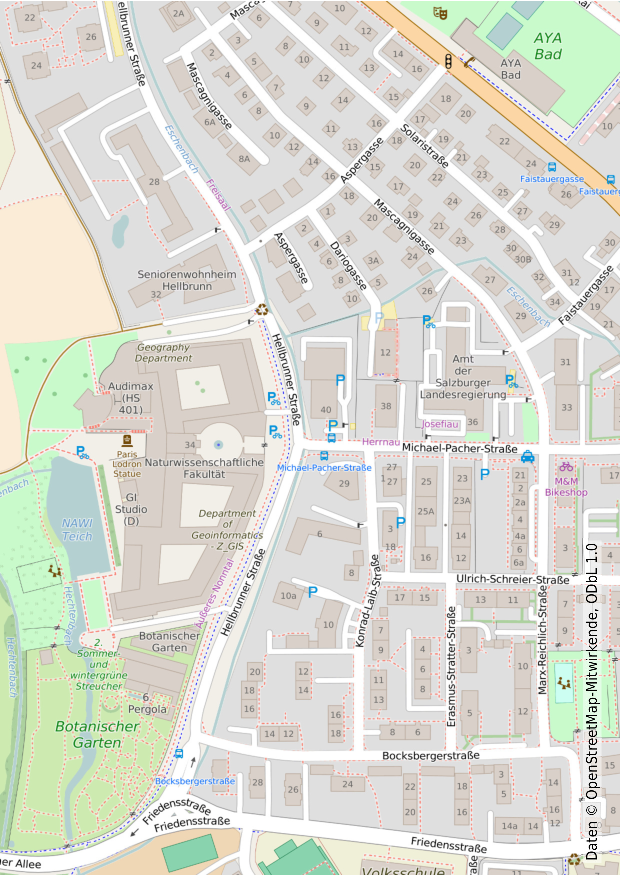
\includepdf{salzburg-campus-karte.pdf}
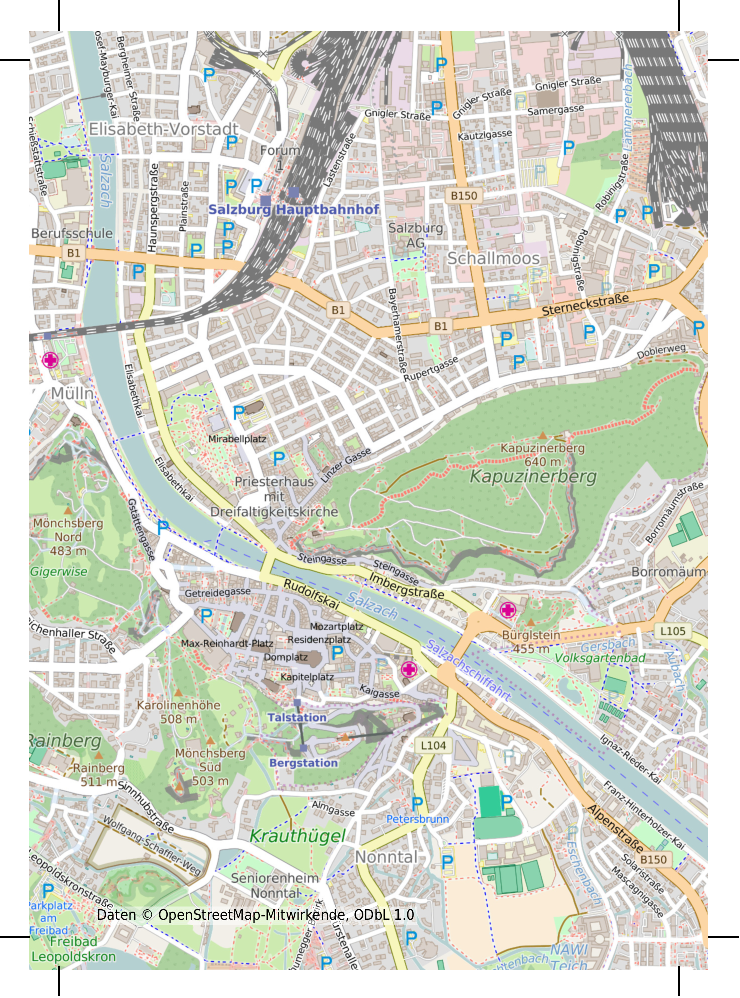
\includepdf{salzburg-uebersicht-karte.pdf}


\end{document}
